\documentclass[hyperref,UTF8]{ctexart}
\usepackage[dvipdfmx]{graphicx}
\usepackage{gbt7714}
\usepackage{float}
\usepackage{ragged2e}
\usepackage{amsthm}
\usepackage{amssymb}
\usepackage{amsmath}
\usepackage{wrapfig}
\usepackage{tikz}
\newtheorem*{proposition}{Ozma Problem}
\usetikzlibrary{arrows.meta}
\newtheorem*{yuzhou}{宇宙}
\usepackage{booktabs}
%\usepackage[a4paper,left=3.18cm,right=3.18cm,top=2.54cm,bottom=2.54cm]{geometry}
\usepackage{tabularx}
\usepackage{array}
\usepackage{caption}
\usepackage{hyperref}
\newcommand{\upcite}[1]{\textsuperscript{\textsuperscript{\cite{#1}}}}
\setCJKfamilyfont{song}{SimSun}
\title{宇宙的方向}
\author{limbo137}
\begin{document}
\maketitle
在地球上,我们可以轻易的判断左右,而在太空中呢?
\section{什么是左右?}
我们常常会有这样的体验,当我们照镜子的时候,我举起左手,镜子里的人就举起右手,也就是说,镜子里的世界是左右颠倒的,换言之,\textbf{镜子把左手“变成”右手}。

%那么事情就好办了,我只要把镜子带上太空,那么就可以随时随地判断左右了

牢记这一点,我们区分的关键就在这里,镜子没办法把我们的头变成脚,但是镜子可以把左手变成右手,用稍微严谨的话来说,\textbf{互为镜像的两类物体区分了空间中的方向}。这话可能有些费解,别担心,待我慢慢道来。

\section{从一维到二维}
想象无垠的宇宙中有一个小点,也只有这一个小点,没有任何的方向可言,但是如果我们经过它画一条直线,然后限定它就在这条直线上运动(如下图)
\[
\begin{tikzpicture}
    \draw[<->] (-2,0)--(2,0);
    \fill (0,0) circle (2pt);
    \node[below left] (O) at (0,0) {$O$};
    \node[below left] (O) at (-2,0) {$\text{左}$};
    \node[below right] (O) at (2,0) {$\text{右}$};
\end{tikzpicture}
\]
它便有了最原始的方向,对它来讲可能就是前进和后退,但在我们看来,这两个方向就是“左”和“右”,如果我们垂直于这条线放置一面镜子,那么很明显,镜子把“左”变成了“右”,假如这条线上存在一种文明,那么它们的语言中,势必会出现代表这两个方向的词,这就是它们的“左”和“右”。

但是我们不满足于此,毕竟这条线上的世界和我们的世界相差还很大。我们给这条线拓展一下,我们找一个可以穿过这条线的平面(这条直线在平面上),在这张平面上生活的文明,就和我们有点像了,虽然我们生活在三维空间,但是因为地球半径太大了,所以我们在地面上很难察觉到地表的弯曲,所以我们如果不计一些地表的起伏,那么我们的地面就可以\textbf{局部地}看作是上面所说的二维平面。(如下图)
\[
\begin{tikzpicture}
    \draw[<->] (-2,0)--(2,0);
    \draw[<->] (0,-2)--(0,2);
    \fill (0,0) circle (2pt);
    \node[below left] (O) at (0,0) {$O$};
    \node[below left] (O) at (-2,0) {$\text{左}$};
    \node[below right] (O) at (2,0) {$\text{右}$};
    \node[below left] (O) at (0,2) {$\text{前}$};
    \node[below right] (O) at (0,-2) {$\text{后}$};
\end{tikzpicture}
\]
我们再来假设一下上面存在的两种生物,第一种生物长这样,我们称之为“右”,理由是如果它以$y$方向为前进方向,那么$x$轴在右边
\[
\begin{tikzpicture}
    \draw[->] (-2,0)--(2,0);
    \draw[->] (0,-2)--(0,2);
    \fill (0,0) circle (2pt);
    \node[below left] (O) at (0,0) {$O$};
    \node[below right] (O) at (2,0) {$\text{x}$};
    \node[below left] (O) at (0,2) {$\text{y}$};
\end{tikzpicture}
\]
第二种生物长这样,我们称之为“左”,理由同上,如果它以$y$方向为前进方向,那么$x$轴在左边
\[
\begin{tikzpicture}
    \draw[<-] (-2,0)--(2,0);
    \draw[->] (0,-2)--(0,2);
    \fill (0,0) circle (2pt);
    \node[below left] (O) at (0,0) {$O$};
    \node[below right] (O) at (-2,0) {$\text{x}$};
    \node[below left] (O) at (0,2) {$\text{y}$};
\end{tikzpicture}
\]
可以看出,第二种是第一种的镜面反射,我们先不论这两种生物是否存在,它们在平面上的运动无非只有两种,平移和旋转,而对于一个“右”来说,无论通过如何的平移和旋转,都无法做到与“左”完全重合,那么我们就把这样的“左”和“右”称为平面的两个\textbf{定向(Orientation)},那我们在二维平面上确定左右的方式如下
\begin{enumerate}
    \item 先选定一个方向作为“前方”
    \item 按照生物“右”的$x$轴指向为右,按照生物“左”的$x$轴指向为左
\end{enumerate}
这里可以看出,左右的定义是依靠一个事先选定的“前方”,换言之这种左右的定义是相对的,但是上面的“左”生物和“右”生物确实绝对的,但是属实没有单一的方向与之对应……真的没有吗?未必,我们对两种生物都让其沿从$x$轴到$y$轴的方向旋转(如下图),
\[
\begin{tikzpicture}
    \draw[->] (-2,0)--(2,0);
    \draw[->] (0,-2)--(0,2);
    \draw[->] (15:1.5) arc [start angle=15, end angle=75, radius=1.5cm];
    \fill (0,0) circle (2pt);
    \node[below left] (O) at (0,0) {$O$};
    \node[below right] (A) at (2,0) {$\text{x}$};
    \node[below left] (B) at (0,2) {$\text{y}$};
\end{tikzpicture},
\begin{tikzpicture}
    \draw[<-] (-2,0)--(2,0);
    \draw[->] (0,-2)--(0,2);
    \fill (0,0) circle (2pt);
    \draw[->] (165:1.5) arc [start angle=165, end angle=105, radius=1.5cm];
    \node[below left] (O) at (0,0) {$O$};
    \node[below right] (O) at (-2,0) {$\text{x}$};
    \node[below left] (O) at (0,2) {$\text{y}$};
\end{tikzpicture}
\]
可以看出,“右”生物的旋转是逆时针的,而“左”生物的旋转是顺时针的,那么两种定向就对应两种旋转方向,这也是一种左右之分,我们通常称之为\textbf{左旋}和\textbf{右旋}。
\section{低维的定向是高维的某个方向}
我们将目光转移到三维空间,也就是我们所在的空间,那么上面的一个“左”生物想要变成一个“右”生物就轻而易举了,我们只需要把它翻转过来,这两个生物就可以完全重合,那么假如这两个生物有正反之分呢?

为了更好的标示二维“左”“右”生物的正反,我们假设存在这样一种三维“右”生物,它长这样
\[
\begin{tikzpicture}
    \draw[->] (-2,0)--(2,0);
    \draw[->] (0,-2)--(0,2);
    \draw[->] (1.6,1.2)--(-1.6,-1.2);
    \fill (0,0) circle (2pt);
    \node[below right] (O) at (0,0) {$O$};
    \node[below right] (O) at (2,0) {$\text{y}$};
    \node[below left] (O) at (0,2) {$\text{z}$};
    \node[below left] (O) at (-1.6,-1.2) {$\text{x}$};
\end{tikzpicture}
\]
可以看出它在二维“右”生物的基础上长出了第三条轴,这其实就是我们平时所说的“右手系”,我们把$z$方向做为三维“右”生物的“正面”,现在“正面”朝上,它对应二维“右”生物,那么当我们翻转它的时候,这个“正面”就会朝下,就会对应二维“左”生物,那么这个“正面”的方向,就可以说是把上面一节中的定向找到了两个实际的方向,但这两个方向在二维平面内是不存在的。

其实,这样的三维“右”生物不是别的,正是我们的右手,还记得我们之前说过的左右旋吗?来,伸出你的右手,先握拳,然后伸出大拇指,让大拇指的方向指向$z$轴,其余四个指头的绕转方向是由$x$到$y$(如图)。
\begin{figure}[H]
    \centering
    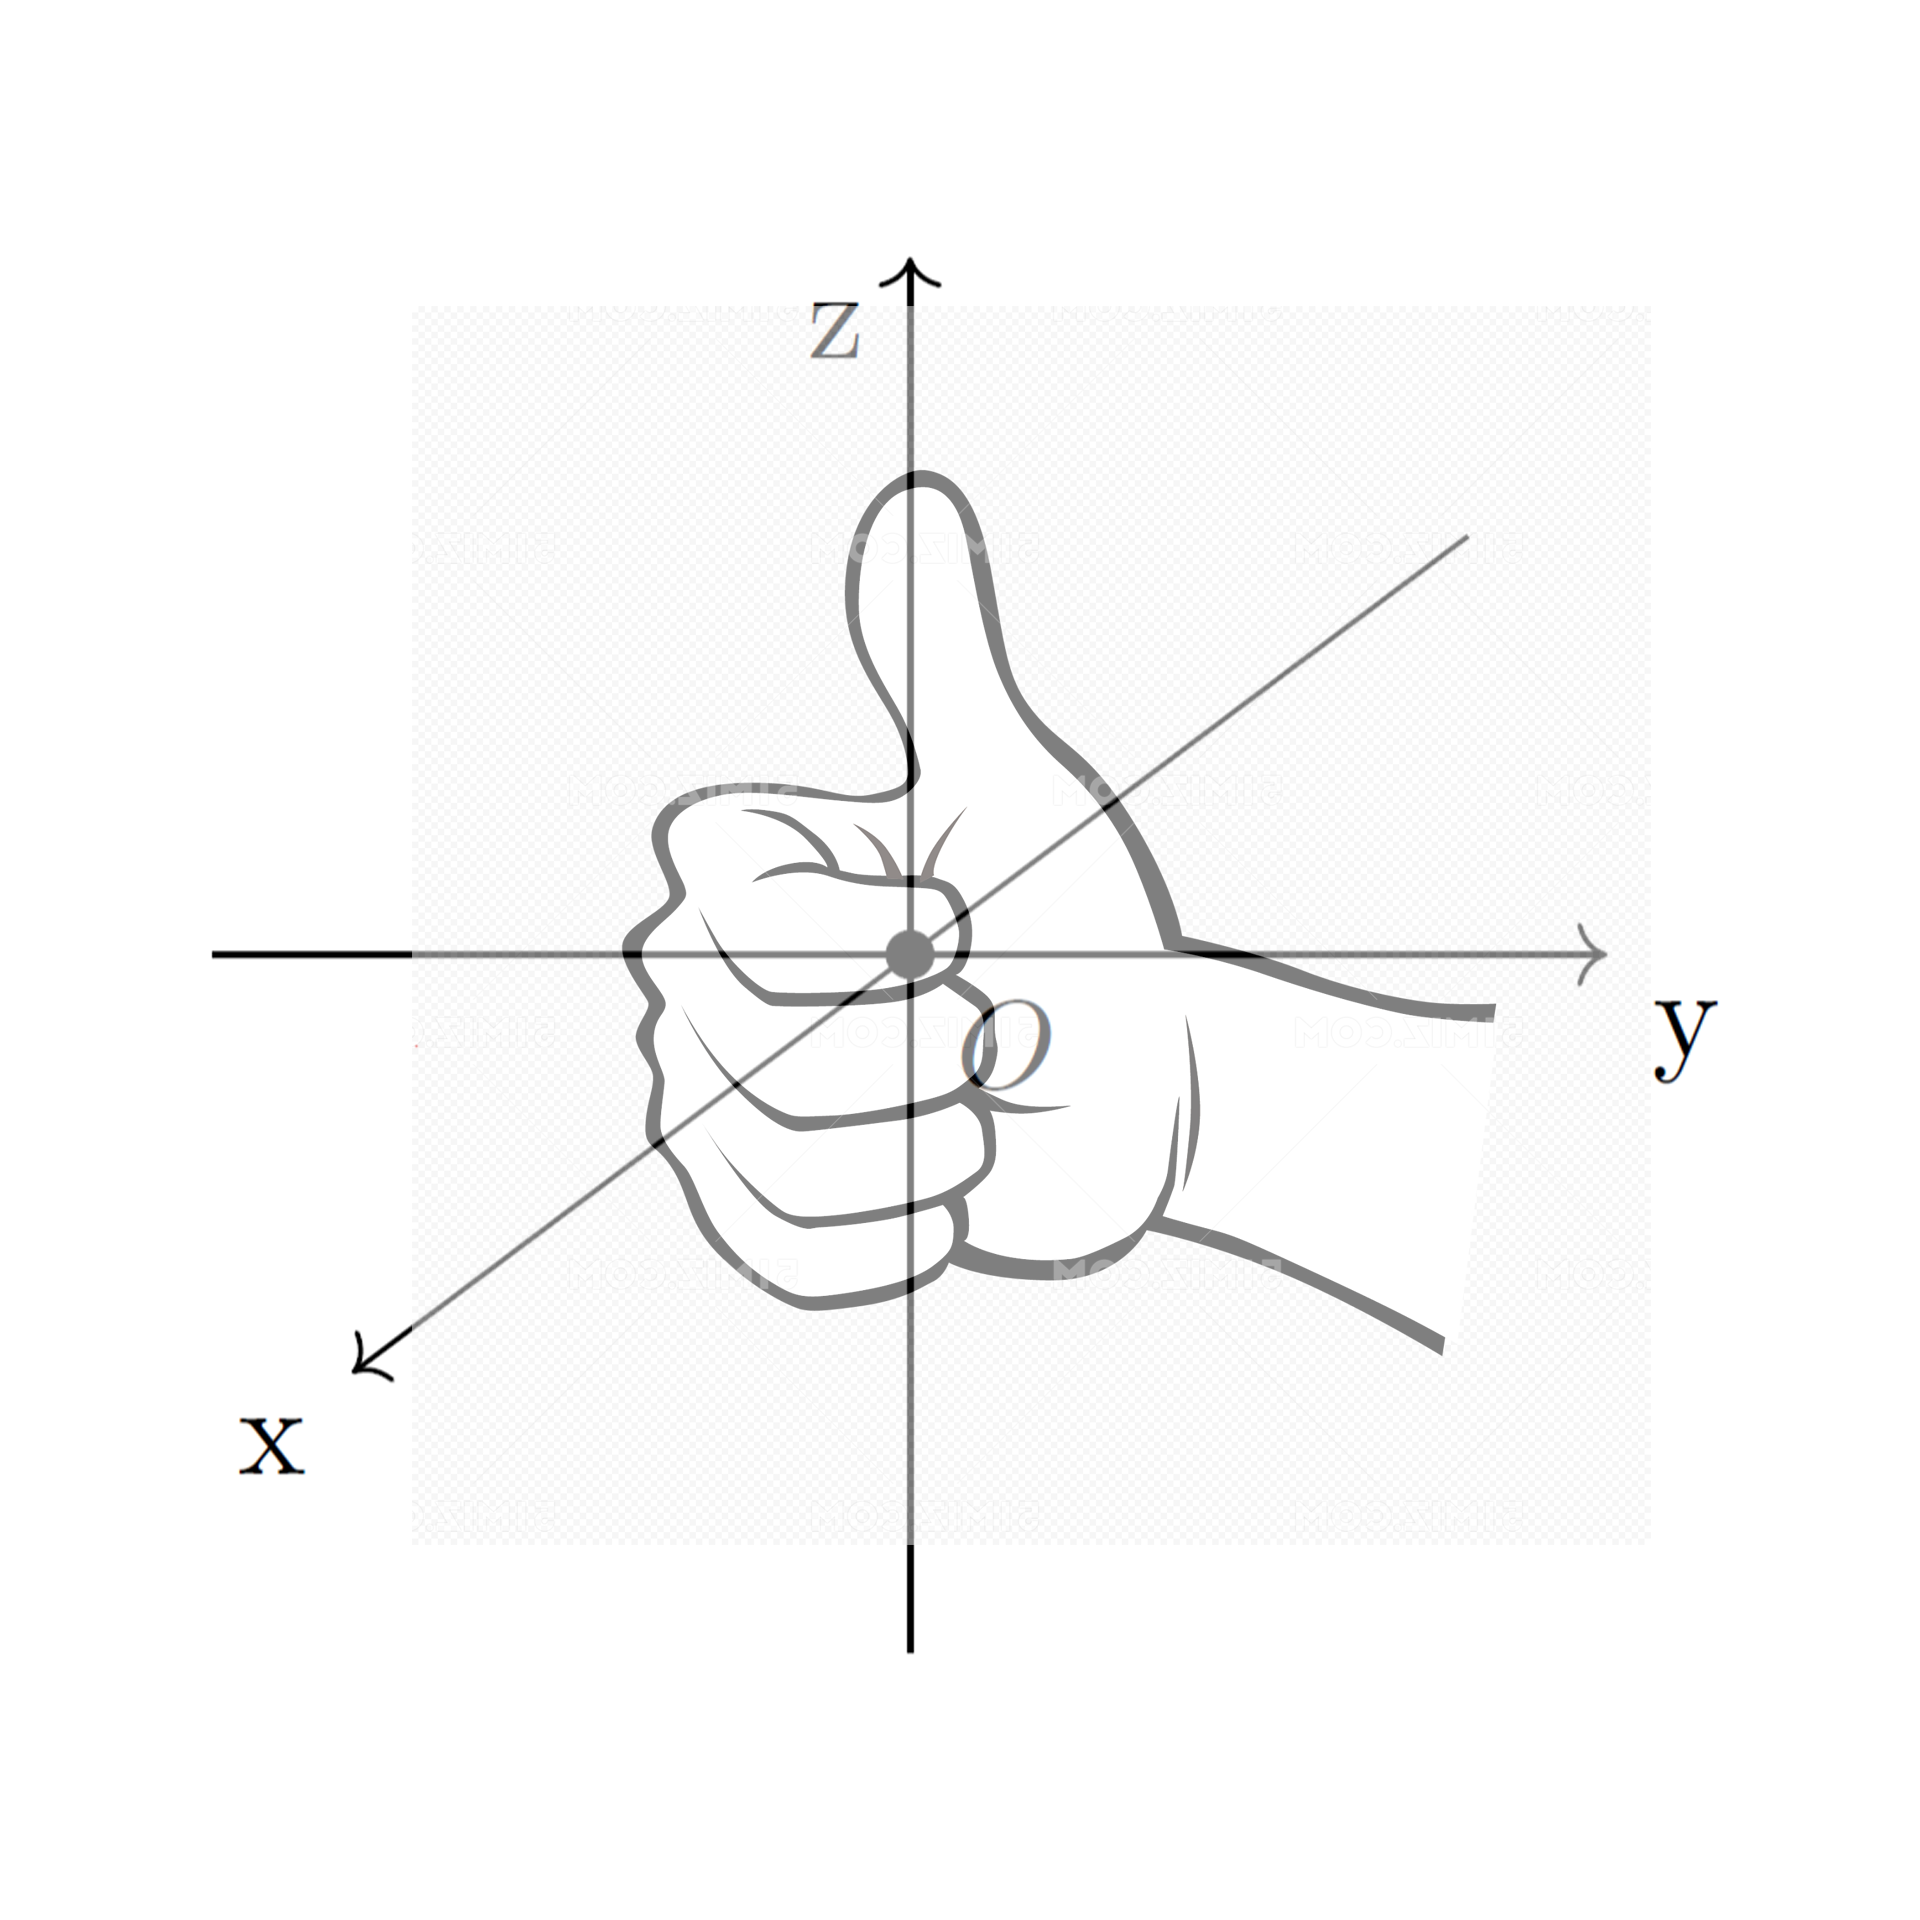
\includegraphics[width=8cm]{大拇指.png}
\end{figure}
按照这种操作,你就可以用右手做出一个三维的“右”生物出来,这里我们看到,其余四指旋转的方向就是上面所说的二维“右”生物的旋转方向,于是通过这样的三维“右”生物,我们把一个\textbf{嵌入}到三维空间中的二维平面(或曲面)确定了定向,这个定向由三维空间中的某个方向(即大拇指方向)确定。

那么现在我们有了三维“右”生物,那么我们是不是也得有个三维“左”生物?只要放面镜子,这“右”生物就变成“左”生物了,对应的也就是我们的左手,于是我们就有了三维空间的两种定向,三维“左”生物和“三维”右生物,它们是互相镜像对称的,不过在物理上,我们更多地称这种镜像对称为\textbf{宇称(Parity)},那么我们就有了在我们的世界真正判断左右的能力,操作如下:
\begin{enumerate}
    \item 首先选定一个方向,作为“上方”
    \item 然后选定一个与上方垂直的方向,作为“前方”
    \item 最后,伸出右手,四指从上方绕到前方,此时大拇指所指的方向,就是右,同理,如果伸出的是左手,那么大拇指所指的方向就是左。
\end{enumerate}
似乎到这里就结束了,我们只要在太空中使用双手判断一下,甚至只用一只手(因为只要判断出右,左就自然确定了),就知道哪边是左,哪边是右了。但是这种做法的前提是,我们假设在太空中判断左右的是一个双手健全(至少有一只)的人类,那么假如一个没有手的生物,例如一个外星人(我们假设它所处的空间也是三维的),它没有地球人“左”“右”的概念,但是它知道三维空间有两种定向,那么我们应该如何告诉它左右的概念呢?换句话说,我们应该如何告诉它怎样从两种生物中挑出三维“右”生物(或“左”生物)?
\section{“上帝是左撇子”}
\begin{figure}[H]
    \centering
    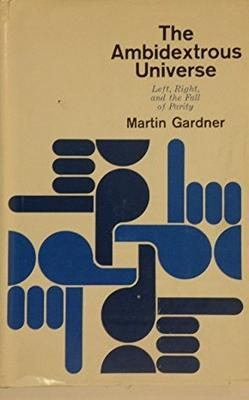
\includegraphics[width=6cm]{TAU.png}
    \caption{《奇妙的宇宙》第一版封面}
\end{figure}
这实际上是一个争论已久的问题,但是所幸现在已经有了结果,这个问题被称为\textbf{奥兹玛问题(Ozma Problem)},最早提出是在1964年马丁·加德纳(Martin Gardner)所著的《灵巧的宇宙》($The$ $Ambidextrous$ $Universe$)一书中,原文的提法翻译过来是
\begin{proposition}
    加德纳声称,如果地球通过奥兹玛项目\footnote{奥兹玛项目是康奈尔大学天文学家弗兰克·德雷克于1960年在西弗吉尼亚州格林银行国家射电天文观测站开始的一项科学实验。实验的目的是通过星际无线电波在遥远的行星系统中寻找生命迹象。名字源于绿野仙踪的衍生作品中的人物奥兹玛公主,是奥兹土地的统领者}与另一个星球上的生命进行交流,就会出现如何交流左和右的定义的问题,其中两个通信者不允许观察任何一个共同的对象。
\end{proposition}
考虑两个实验室,两个实验室完全镜像对称,那么它们所做的同一个物理实验,按照我们的直觉,结果应该也是对称的,这也是上面的问题难以解决的症结所在,这个问题首先隐含在伊曼纽尔·康德关于孤立在空间中的手的讨论中,这个手就像我们前面所述的“左”生物或是“右”生物,因为它们只有互相对照才能区别,否则这只手本身没有左右意义。

但是在1956年,中国科学家吴健雄就在实验上说明,$\beta$衰变过程(可以理解为中子变为质子和电子的过程,我们一般称之为\textbf{弱相互作用(weak interacyions)})中,对称的实验条件并不能导致相同的结果,这一结论称为\textbf{宇称不守恒(P symmetry violation)},由杨振宁和李政道提出,他们也因此获得1957年诺贝尔物理学奖。
\begin{figure}[H]
    \centering
    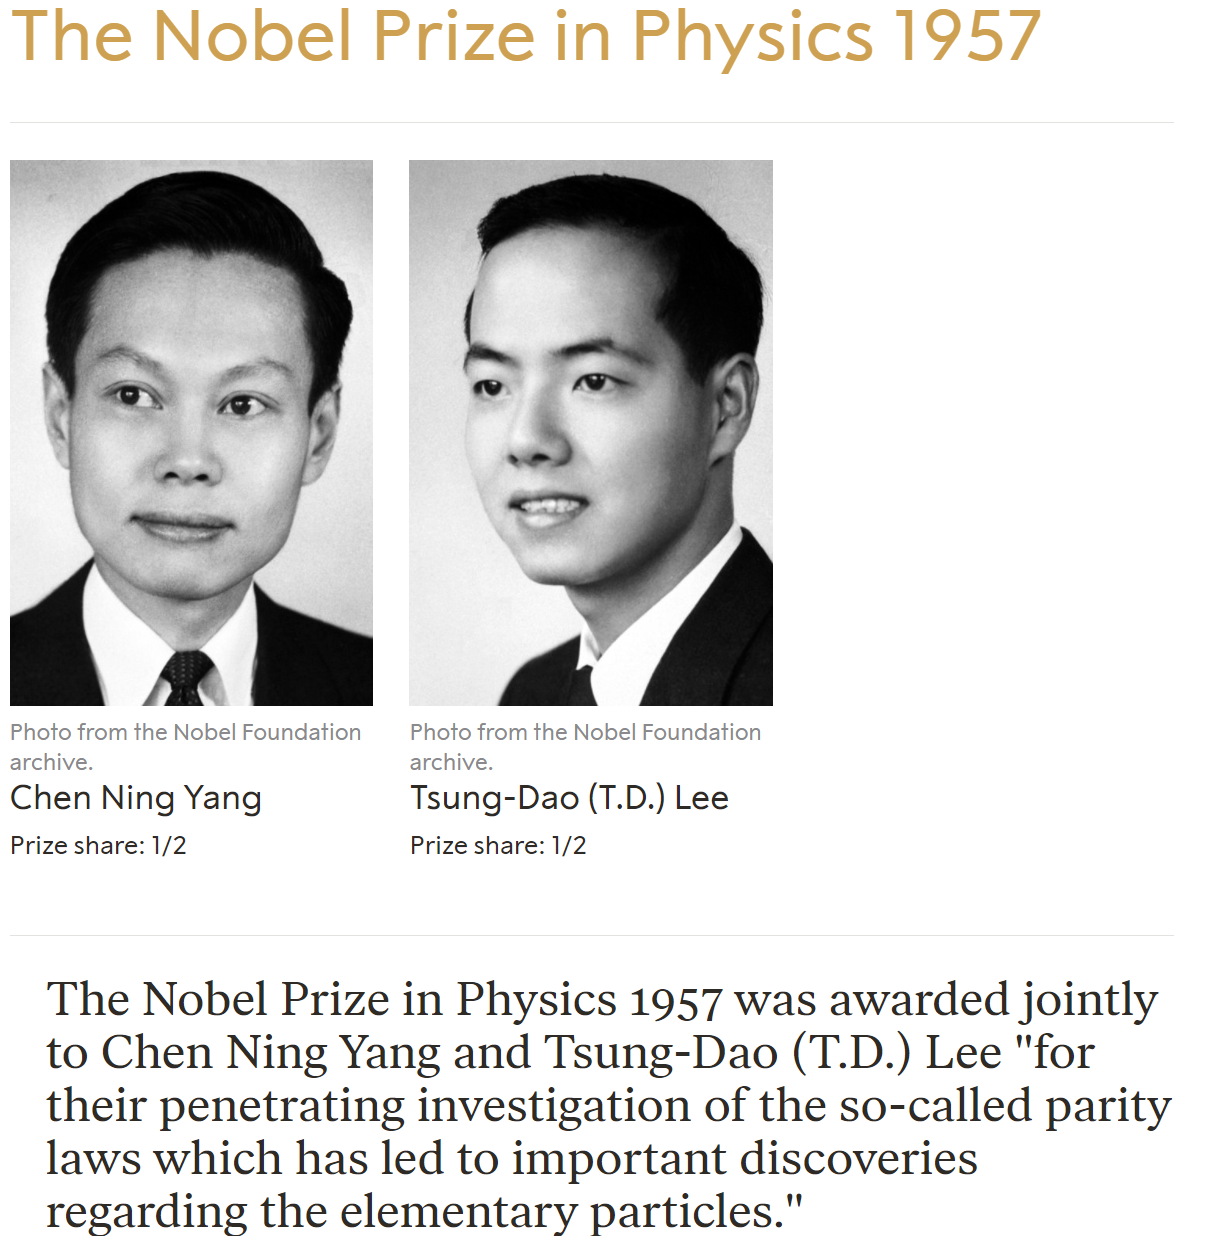
\includegraphics[width=5cm]{屏幕截图 2021-10-01 205815.png}
    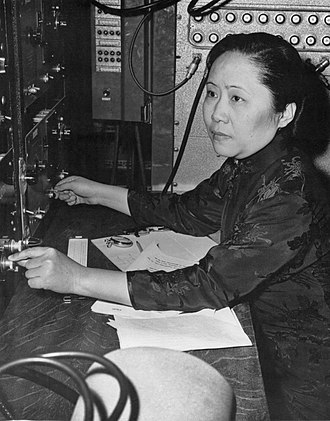
\includegraphics[width=4cm]{330px-Chien-shiung_Wu_(1912-1997)_C.jpg}
    \caption{左为杨振宁和李政道,右为吴健雄(图片来源:维基百科)}
\end{figure}
我们有必要仔细谈谈这个实验,它被命名为吴氏实验,吴健雄使用了完全镜像对称的两个体系,发现反应后射出的电子在平行与镜面的方向上相反了,它们本来应该放出方向一致的电子,这个实验的结果轰动一时,因为这个结果就意味着上面的“左”生物和“右”生物并不是完全对称的,也就是说,大自然对其中一种定向有偏向性,这个结论也常常被称为“上帝是左撇子”,这个结果的意义之大可想而知。
\begin{figure}[H]
    \centering
    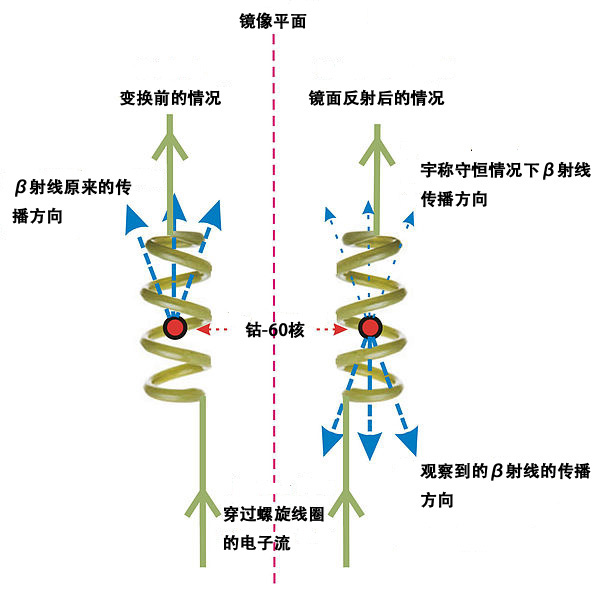
\includegraphics[width=6cm]{Parity_violation_principle_Wu_experiment_(zh-hans).jpg}
    \caption{镜像对称后,本不该反向的$\beta$射线(即电子流)反向了(图片来源:维基百科)}
\end{figure}
观察上面的图,虽然我们可能并不了解其中的原理,但是可以伸出左手比划一下,让四指的绕向和螺线管中电流方向相同,此时大拇指所指的方向就是电子(也就是$\beta$射线)的传播方向,你会惊讶的发现,左边的图和右边的图虽然镜像对称,但是实际上它们对应左手!这便是上帝的“神之左手”。

到此为止,我们就可以解决前面提到的奥兹玛问题了,虽然规定不能观察同一个对象,但是由于上帝是左撇子,那么就有一个天生的“神之左手”,这个左手就是吴氏实验,我们只要让外星人复现吴氏实验,那么我们就可以让他们称这种定向为“左”,那么另一种定向“右”也就确定了,奥兹玛问题也就迎刃而解了。

到这里就真正结束了吗?似乎还没有,我们并没有解释为什么大自然会偏向这个定向。
\section{CPT联合对称}
我们在第三节说过,低维的定向是高维的某个方向,这个方向是低维看不到的,那么如果在三维有一个特殊定向的话,就应该昭示四维有一个特殊的方向,这其实并不稀奇,我们的所处的宇宙其实并不是三维的,我们来看看古人如何定义宇宙
\begin{yuzhou}
    上下四方曰宇,古往今来曰宙
\end{yuzhou}
我们刚刚只是一直在关注“上下四方”而并没有关注“古往今来”,也就是说,我们忽略了时间,如果把时间加上,我们就生活在一个\textbf{四维时空(Four Dimensional Space-Time)}当中,三维空间中的定向就可以与四维空间中的两个时间方向,过去和将来,相对应。准确的说是时间指向过去还是将来,我们知道时间是一直向前,不会向后的,那么时间的方向就已经不是镜像对称的了,既然与三维定向相对应的时间方向都不对称,那两个三维定向对称反倒才是怪事,虽然这么说,但是我们所处的世界在大部分情况下两个定向还是对称的。虽然宇称不再守恒,但是把体系镜像之后,再把时间轴也反向(一般我们称之为时间反演),体系依然是对称的,这个操作称为\textbf{PT联合对称},但是其实还不够,我们在基本粒子中,还存在电荷的反向,从正电荷到负电荷的变换,其实这种变换还可以推广到正物质和反物质的变换,这种变换下不变则成为\textbf{C对称},现代物理学认为,CPT必须具有联合对称性,即在镜像,时间反演,和正反物质变换过后,世界应该是完全一样的(也就是对称的)。但是这个定理的正确性还要等待时间去证明。

很多物理学都建立在对称与守恒的基础上,对称的发现和打破都是物理学中的大事,虽然我们的一开始的目的是为了在宇宙中探究左右,但是科学的发展往往将一些不相关的领域连起来,所以我们到这里也并不奇怪,大自然本就是相互关联的。

写在最后,笔者的水平有限,若有纰漏和谬误,欢迎指出。
\end{document}